% ******************************* PhD Thesis Template **************************
% Please have a look at the README.md file for info on how to use the template

\documentclass[a4paper,12pt,numbered,print,index,custommargin, oneside]{Classes/PhDThesisPSnPDF}

% ******************************************************************************
% ******************************* Class Options ********************************
% *********************** See README for more details **************************
% ******************************************************************************

% `a4paper'(The University of Cambridge PhD thesis guidelines recommends a page
% size a4 - default option) or `a5paper': A5 Paper size is also allowed as per
% the Cambridge University Engineering Deparment guidelines for PhD thesis
%
% `11pt' or `12pt'(default): Font Size 10pt is NOT recommended by the University
% guidelines
%
% `oneside' or `twoside'(default): Printing double side (twoside) or single
% side.
%
% `print': Use `print' for print version with appropriate margins and page
% layout. Leaving the options field blank will activate Online version.
%
% `index': For index at the end of the thesis
%
% `draftclassic': For draft mode without loading any images (same as draft in book)
%
% `draft': Special draft mode with line numbers, images, and water mark with
% timestamp and custom text. Position of the text can also be modified.
%
% `abstract': To generate only the title page and abstract page with
% dissertation title and name, to submit to the Student Registry
%
% `chapter`: This option enables only the specified chapter and it's references
%  Useful for review and corrections.
%
% ************************* Custom Page Margins ********************************
%
% `custommargin`: Use `custommargin' in options to activate custom page margins,
% which can be defined in the preamble.tex. Custom margin will override
% print/online margin setup.
%
% *********************** Choosing the Fonts in Class Options ******************
%
% `times' : Times font with math support. (The Cambridge University guidelines
% recommend using times)
%
% `fourier': Utopia Font with Fourier Math font (Font has to be installed)
%            It's a free font.
%
% `customfont': Use `customfont' option in the document class and load the
% package in the preamble.tex
%
% default or leave empty: `Latin Modern' font will be loaded.
%
% ********************** Choosing the Bibliography style ***********************
%
% `authoryear': For author-year citation eg., Krishna (2013)
%
% `numbered': (Default Option) For numbered and sorted citation e.g., [1,5,2]
%
% `custombib': Define your own bibliography style in the `preamble.tex' file.
%              `\RequirePackage[square, sort, numbers, authoryear]{natbib}'.
%              This can be also used to load biblatex instead of natbib
%              (See Preamble)
%
% **************************** Choosing the Page Style *************************
%
% `default (leave empty)': For Page Numbers in Header (Left Even, Right Odd) and
% Chapter Name in Header (Right Even) and Section Name (Left Odd). Blank Footer.
%
% `PageStyleI': Chapter Name next & Page Number on Even Side (Left Even).
% Section Name & Page Number in Header on Odd Side (Right Odd). Footer is empty.
%
% `PageStyleII': Chapter Name on Even Side (Left Even) in Header. Section Number
% and Section Name in Header on Odd Side (Right Odd). Page numbering in footer

% ********************************** Preamble **********************************
% Preamble: Contains packages and user-defined commands and settings
% ******************************************************************************
% ****************************** Custom Margin *********************************

% Add `custommargin' in the document class options to use this section
% Set {innerside margin / outerside margin / topmargin / bottom margin}  and
% other page dimensions
\ifsetCustomMargin
  \RequirePackage[left=30mm,right=25mm,top=25mm,bottom=25mm]{geometry}
  \setFancyHdr % To apply fancy header after geometry package is loaded
\fi

% Add spaces between paragraphs
%\setlength{\parskip}{1em} - see after \begin{document}

% Ragged bottom avoids extra whitespaces between paragraphs
\raggedbottom
% To remove the excess top spacing for enumeration, list and description
%\usepackage{enumitem}
%\setlist[enumerate,itemize,description]{topsep=0em}

% *****************************************************************************
% ******************* Fonts (like different typewriter fonts etc.)*************

% Add `customfont' in the document class option to use this section

\ifsetCustomFont
  % Set your custom font here and use `customfont' in options. Leave empty to
  % load computer modern font (default LaTeX font).
  %\RequirePackage{helvet}

  % For use with XeLaTeX
  %  \setmainfont[
  %    Path              = ./libertine/opentype/,
  %    Extension         = .otf,
  %    UprightFont = LinLibertine_R,
  %    BoldFont = LinLibertine_RZ, % Linux Libertine O Regular Semibold
  %    ItalicFont = LinLibertine_RI,
  %    BoldItalicFont = LinLibertine_RZI, % Linux Libertine O Regular Semibold Italic
  %  ]
  %  {libertine}
  %  % load font from system font
  %  \newfontfamily\libertinesystemfont{Linux Libertine O}
\fi

% *****************************************************************************
% **************************** Custom Packages ********************************

% ************************* Algorithms and Pseudocode **************************

\usepackage{algpseudocode}


% ********************Captions and Hyperreferencing / URL **********************

% Captions: This makes captions of figures use a boldfaced small font.
\RequirePackage[small,bf]{caption}

\RequirePackage[,tableposition=top]{caption} % labelsep=space for space 
\renewcommand{\figurename}{Figure} %to support older versions of captions.sty

% *************************** Graphics and figures *****************************

%\usepackage{rotating}
%\usepackage{wrapfig}

% Uncomment the following two lines to force Latex to place the figure.
% Use [H] when including graphics. Note 'H' instead of 'h'
\usepackage{graphbox}
\usepackage{float}
\restylefloat{figure}

% Subcaption package is also available in the sty folder you can use that by
% uncommenting the following line
% This is for people stuck with older versions of texlive
%\usepackage{sty/caption/subcaption}
\usepackage{subcaption}

% ********************************** Tables ************************************
\usepackage{booktabs} % For professional looking tables
\usepackage{multirow}

\usepackage{multicol}
\usepackage{longtable}
\usepackage{tabularx}
\usepackage{parskip}

% *********************************** SI Units *********************************
\usepackage{siunitx} % use this package module for SI units


% ******************************* Line Spacing *********************************

% Choose linespacing as appropriate. Default is one-half line spacing as per the
% University guidelines

% \doublespacing
% \onehalfspacing
% \singlespacing


% ************************ Formatting / Footnote *******************************

% Don't break enumeration (etc.) across pages in an ugly manner (default 10000)
\clubpenalty=500
\widowpenalty=500

\usepackage[bottom]{footmisc} 
% `perpage`: Range of footnote options, reset to 1 per page
% `bottom`: sticks footnote to the end of page regardless



% *****************************************************************************
% *************************** Bibliography  and References ********************

%\usepackage{cleveref} %Referencing without need to explicitly state fig /table

% Add `custombib' in the document class option to use this section
\ifuseCustomBib
%   \RequirePackage[square, sort, numbers, authoryear]{natbib} % CustomBib

% If you would like to use biblatex for your reference management, as opposed to the default `natbibpackage` pass the option `custombib` in the document class. Comment out the previous line to make sure you don't load the natbib package. Uncomment the following lines and specify the location of references.bib file

\RequirePackage[backend=biber, style=numeric-comp, citestyle=numeric, sorting=nty, natbib=true]{biblatex}
\addbibresource{References/references} %Location of references.bib only for biblatex, Do not omit the .bib extension from the filename.
\fi

% changes the default name `Bibliography` -> `References'
%\renewcommand{\bibname}{References}


% ******************************************************************************
% ************************* User Defined Commands ******************************
% ******************************************************************************

% *********** To change the name of Table of Contents / LOF and LOT ************

\renewcommand{\contentsname}{Contents}
%\renewcommand{\listfigurename}{My List of Figures}
%\renewcommand{\listtablename}{My List of Tables}


% ********************** TOC depth and numbering depth *************************

% Uncomment the next 2 lines to add dots to TOC
%\usepackage{tocloft}  
%\renewcommand{\cftchapleader}{\cftdotfill{\cftdotsep}} 
\setcounter{secnumdepth}{2}
\setcounter{tocdepth}{2}


% ******************************* Nomenclature *********************************

% To change the name of the Nomenclature section, uncomment the following line

%\renewcommand{\nomname}{Symbols}


% ********************************* Appendix ***********************************

% The default value of both \appendixtocname and \appendixpagename is `Appendices'. These names can all be changed via:

%\renewcommand{\appendixtocname}{List of appendices}
%\renewcommand{\appendixname}{Appndx}
\usepackage{docmute} % only needed to allow inclusion of proposal.tex

% *********************** Configure Draft Mode **********************************

% Uncomment to disable figures in `draft'
%\setkeys{Gin}{draft=true}  % set draft to false to enable figures in `draft'

% These options are active only during the draft mode
% Default text is "Draft"
%\SetDraftText{DRAFT}

% Default Watermark location is top. Location (top/bottom)
%\SetDraftWMPosition{bottom}

% Draft Version - default is v1.0
%\SetDraftVersion{v1.1}

% Draft Text grayscale value (should be between 0-black and 1-white)
% Default value is 0.75
%\SetDraftGrayScale{0.8}


% ******************************** Todo Notes **********************************
%% Uncomment the following lines to have todonotes.

%\ifsetDraft
%	\usepackage[colorinlistoftodos]{todonotes}
%	\newcommand{\mynote}[1]{\todo[author=kks32,size=\small,inline,color=green!40]{#1}}
%\else
%	\newcommand{\mynote}[1]{}
%	\newcommand{\listoftodos}{}
%\fi

% Example todo: \mynote{Hey! I have a note}

% *****************************************************************************
% ******************* Better enumeration my MB*************
\usepackage{enumitem}

% ************************ Thesis Information & Meta-data **********************
% Thesis title and author information, refernce file for biblatex
% ************************ Thesis Information & Meta-data **********************
%% The title of the thesis
\title{An accelerated, network-assisted TCP recovery}

%% Subtitle (Optional)
\subtitle{Computer Science Tripos - Part II Project Proposal}

%% The full name of the author
\author{Thanh Bui}

%% Department (eg. Department of Engineering, Maths, Physics)
\dept{Department of Computer Science}

%% University and Crest
\university{University of Cambridge}

% Crest minimum should be 30mm.
\crest{
\includegraphics[width=0.3\textwidth]{University_Crest}}

%% Supervisor (optional)
\supervisor{Dr Noa Zilberman}

%% College affiliation (optional)
\college{Downing College}

%% Submission date
\degreedate{October 19, 2018} 

%% Meta information
\subject{LaTeX} \keywords{{LaTeX} {PhD Thesis} {Engineering} {University of
Cambridge}}


\begin{document}
\setlength{\parskip}{0.75\baselineskip}

\maketitle

% ******************************** Main Proposal *********************************

\chapter{Introduction}
\textit{In this chapter, I provide the motivation for this project and setup the problem I am solving. I also explain some key algorithms involved. Finally, I cover some related work.}

\section{Motivation}
	
 Transmission Control Protocol (TCP) is the protocol of choice in many data centers. However, it is very sensitive to losses (by design, as a mean for congestion control), which can degrade the performance within the data centers significantly \cite{zilberman2017has}. Various congestion control, avoidance and recovery mechanisms are thus of high importance in this field to minimise such loss rate. Still, not all TCP losses are born equal. For example, losses happening at the destination host's network interface card (NIC) are not an indication of congestion within the network. It is assumed that fast retransmission of such lost packets, from within the network, can increase the utilization of the network.
 
 In-network computing is an emerging research area in systems and networking, where applications traditionally running on the host are offloaded to the network hardware (e.g. switch, NIC). Examples of applications offloaded in the past include network functions (DNS server \cite{dns}), distributed systems functions such as consensus (P4xos \cite{p4xos}), various caching (netCache \cite{netCache}, netChain \cite{netChain}) and even a game (Tic-Tac-Toe). Key-Value Store (KVS) is also among the popular type of in-network applications. 
 
 Therefore, it is particularly interesting, and indeed challenging, to see how network-accelerated KVS concepts can be applied to TCP fast retransmit mechanism in order to improve cross-datacentre performance.
 
\section{Project Aims}
Fast retransmit is an enhancement to TCP that reduces the time a sender waits before retransmitting a lost segment. A TCP sender normally uses a simple timer to recognize lost segments. If an acknowledgement is not received for a particular segment within a specified time (a function of the estimated round-trip delay time), the sender will assume the segment was lost in the network, and will retransmit the segment.

Duplicate acknowledgement (DUP ACK) is the basis for the fast retransmit mechanism. After receiving a packet (e.g. with sequence number 1), the receiver sends an acknowledgement by adding 1 to the sequence number (i.e. acknowledgement number 2). This indicates to the sender that the receiver received the packet number 1 and it expects packet number 2. Suppose that three subsequent packets are lost. The next packets the receiver sees are packet numbers 5 and 6. After receiving packet number 5, the receiver sends an acknowledgement, but still only for sequence number 2. When the receiver receives packet number 6, it sends yet another acknowledgement value of 2. Duplicate acknowledgement occurs when the sender receives more than one acknowledgement with the same sequence number (2 in our example).

When a sender receives several DUP ACKs, it can be reasonably confident that the segment with the sequence number specified in the DUP ACK was dropped. A sender with fast retransmit will then retransmit this packet immediately without waiting for its timeout.

\begin{figure}[h]
	\centering
	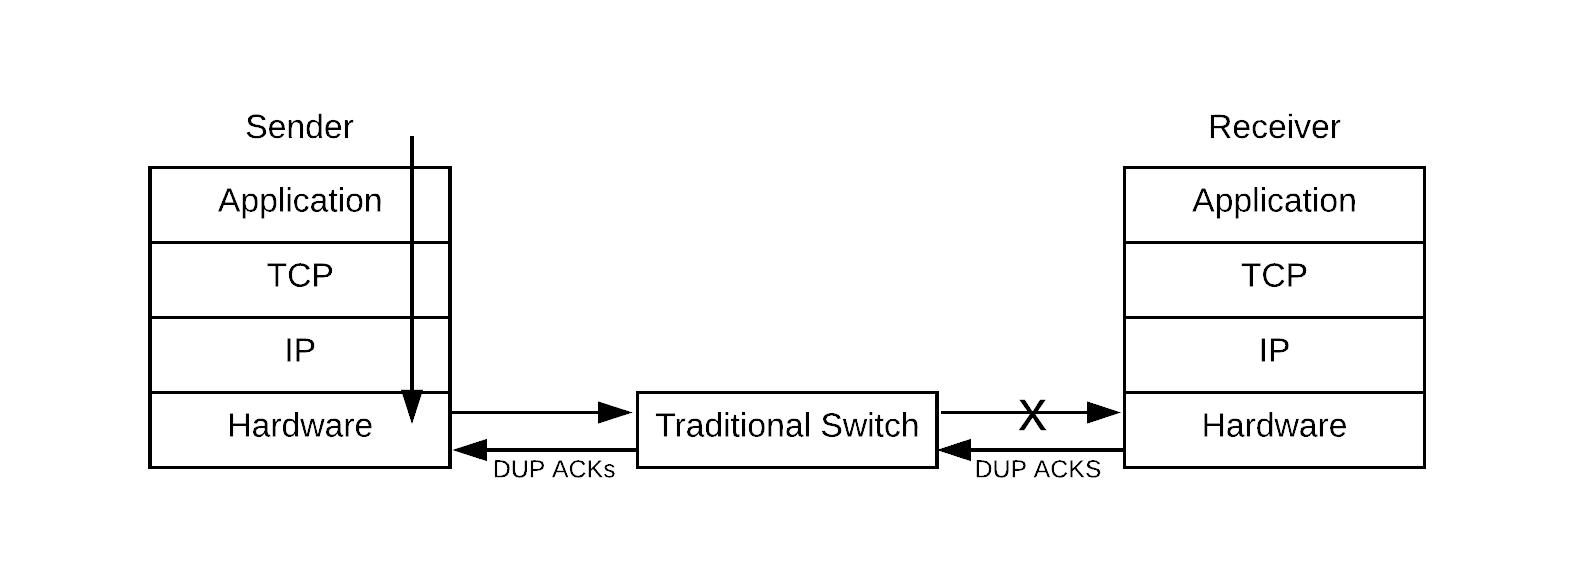
\includegraphics[width=\textwidth]{tradition-tcp.png}
	\caption{The standard convention of TCP handling.}
	\label{tradition-tcp}
\end{figure}

Currently, the DUP ACKs will traverse all the way back to the sender (\textbf{Figure \ref{tradition-tcp}}). The sender receives the DUP ACKs, then retransmits the packet with the next higher sequence number. 

\begin{figure}[h]
	\centering
	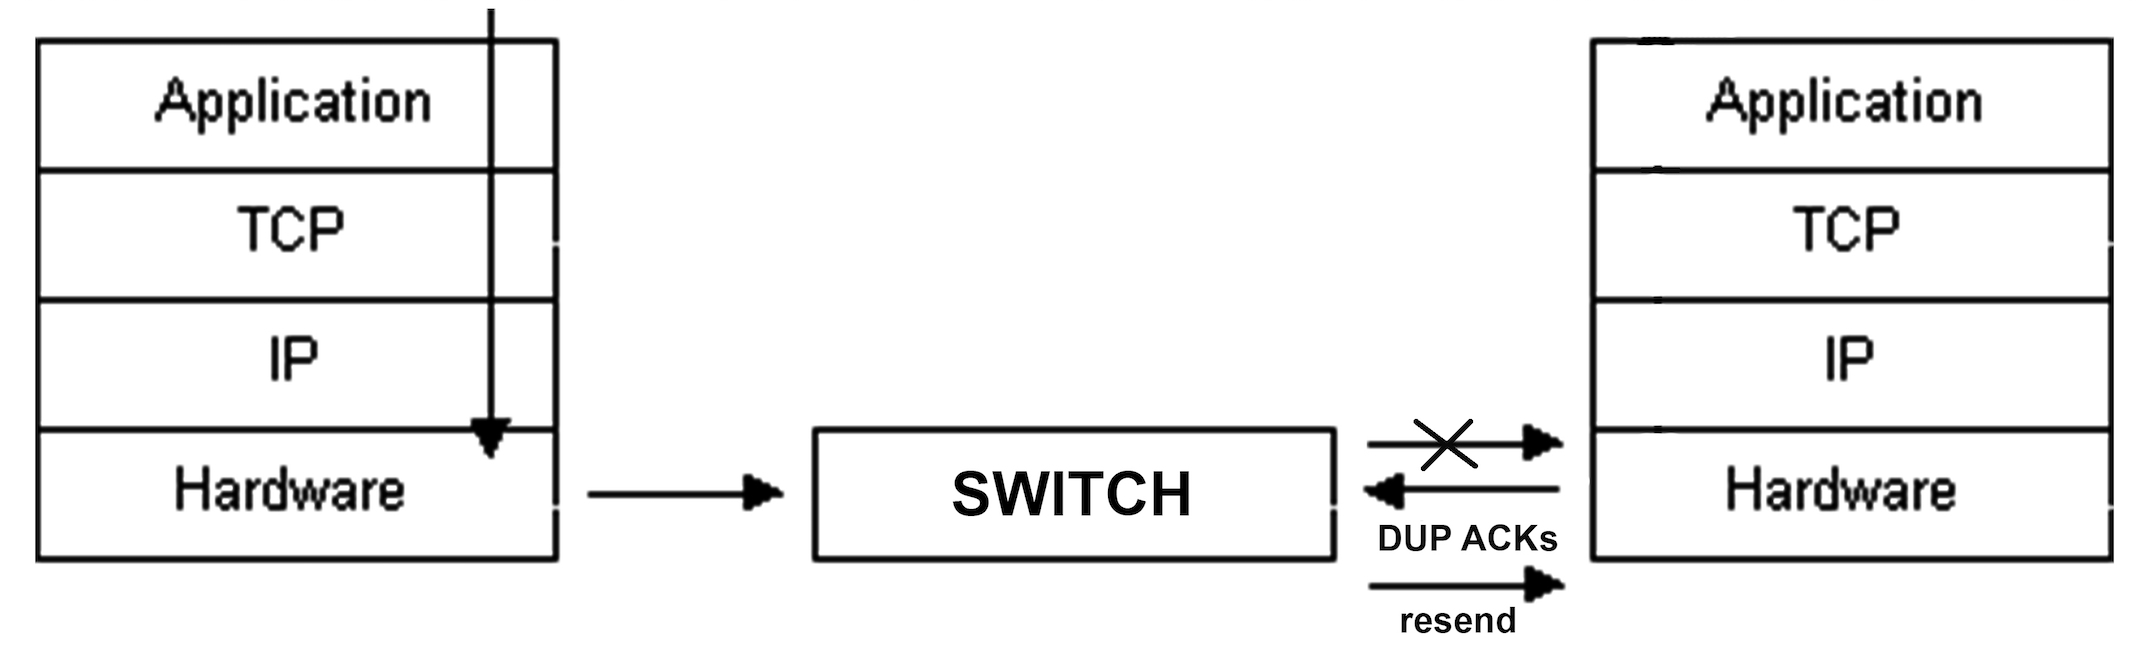
\includegraphics[width=\textwidth]{project-tcp.png}
	\caption{The proposed TCP handling.}
	\label{project-tcp}
\end{figure}

This project aims to design and implement a programmable switch that assists the TCP fast retransmit algorithm. The programmable switch will be able to retransmit the packets from within the network, instead of waiting for the DUP ACKs to get back to the host (\textbf{Figure \ref{project-tcp}}), thereby aims to reduce the response time to DUP ACKs and reduce unnecessary changes to the congestion window. The implementation will be based on the KVS concept, where the keys are the flow ID and the packet sequence number, and the value is the payload.

\section{Related Work}
	\subsection{TCP Congestion Control}
	One of the main aspects of TCP is congestion control, where a number of mechanisms are used to achieve high performance and avoid sending more data than the network is capable of forwarding, that is, to avoid causing network congestion. In particular, TCP uses a \textit{congestion avoidance} algorithm that includes various aspects of an additive increase/multiplicative decrease (AIMD) scheme, with other schemes such as \textit{slow start}, \textit{fast retransmit} and \textit{fast recovery} to achieve congestion avoidance. 
	
	The four intertwined algorithms are defined in more detail in RFC 5681\cite{rfc5681}. In this project, we are mostly interested in the \textit{fast retransmit} algorithm, which has been explained in the previous section.
	
	\subsection{Programmable Data Planes}
	The use of P4, netFPGA, etc.


\section*{\fontsize{18pt}{0.5}\selectfont Starting Point}

\subsection*{Platform \& Language}
This project will work mainly with a NetFPGA SUME board \cite{netfpgasume}, using P4 programming language. I will be using the P4-NetFPGA workflow, which provides infrastructure to compile P4 programs to NetFPGA \cite{fpga}. Apart from that, everything else will be built from scratch.

I have no prior experience with either NetFPGA or P4, but this will be mitigated through self-learning in which I will make use of the online tutorials, Google's resources and the P4 community documentation, as well as the experience of my supervisors. 

\subsection*{Computer Science Tripos}
The relevant Tripos courses that can serve as a starting point for this project are primarily: \emph{Computer Networking}, \emph{Principles of Communications} and \emph{ECAD and Architecture Practical Classes}. Since the courses are introductory, I will also consult Part III's \emph{High Performance Networking} course. I also plan to bridge any knowledge gap through extensive personal reading as well as help from my project supervisor.
\section*{\fontsize{18pt}{1}\selectfont Resources Required}

For this project I will be using my own computer, a 2017 MacBook Pro with a 2.3 GHz Intel Core i5 processor and 16 GB of RAM, that runs macOS Mojave. I accept full responsiblity for this machine, and I have made contingency plans to deal with hardware and/or software failures. Should that machine suddenly fail, I have another 16Gb of RAM computer with a 2.6 GHz Intel Core i7 processor that runs Ubuntu 18.04 LTS. If all else fails, I can continue to work on an MCS machine. Backups will be done weekly to Microsoft OneDrive and my external hardrive, and all my codes will be uploaded to GitHub for version control. 

For the hardware prototype, I will require a NetFPGA SUME board. I will need access to a machine that has the SUME installed, and a 10G NIC. These will be supplied by my supervisor. I will be using my own machine for development, with remote access to a server with the SUME board inside.

I will also require access to the lab network in order to \emph{ssh} to the server with the SUME board. Development on my machine will require VPN access, for using floating licenses of the development tools. Lastly, I will require a second server for testing some of the extensions of the project.
\section*{\fontsize{18pt}{1}\selectfont Work to be Done}

The main core component of the project is to be able to apply the KVS concept, where the sequence number and flow Id of a packet are the key and the packet is the value, to implement TCP fast recovery. In order to do that, the following sub-tasks must be done:

\begin{enumerate}
	
	\item First, since the project is done on NetFPGA using P4 programming language, both of which I am not familar with, I first have to study them thoroughly and be proficient working with the platform.
	
	\item I would also need to study and gain a better understanding of KVS applications, TCP congestion control and recovery mechanisms, as well as their use cases (e.g. High Frequency Trading, in-datacenter latency sensitive applications, etc.).
	
	\item The next stage will be to design the architecture for the application. This is a non-trivial process. Generally, it will be to try to map the application to a match-action pipeline.
	
	\item The fourth stage involves implementing the architecture in code. The program, which will be written in P4, will have the basic functionalities such as:
	\begin{itemize}
		\item A basic L3 switch function and TCP decoding (send TCP, read the flow information from the table/register)
		
		\item Matching packets to a "\emph{key}" (its flow Id):
			\begin{itemize}
				\item If the key is of a new packet, store it (SET()).
				\item If the key is of a DUP ACK, read the packet and re-send (GET()).
				\item If the number of DUP ACKs is greater than $N$, do not resend. Instead, forward to host as the standard convention of handling TCP.
				\item Do not resend if the flow Id is not in a "selected" table. In other words, use the KVS only if the flow Id matches a predefined set of flow Ids, or a different predefined rule by the user.
			\end{itemize}		
	
	\end{itemize}
	
	\item \textbf{The simulation stage:} perform functionality test by simulating the program using bmv2 or Xilinx simulators to ensure correctness. 
	
	\item After it runs smoothly in the software, it will then be compiled to the hardware. Ensure that the basic functionalities mentioned above work in hardware.
	
	\item \textbf{The hardware stage:} demonstrate interoperability with a software-based client/application.
	
	Possibly, I will implement a drop $1:N$ packets at the server to force DUP ACKs, and I will also be using a synthetic benchmark such as \emph{multilate} \cite{multilate} -- a memcached benchmark -- or OSNT \cite{OSNT} as the applications on top of the network. The criterion to evaluate the performance is the flow completion time. There is no intention to use network simulators such as ns2, omnet++, etc. This is outside the scope of this project.
	
	The aim for this stage is to get a working prototype in hardware that supports a single flow and single packet size, and evaluate on its performance.
	
	\item Once the prototype is up and working, I need to implement further extensions to allows the prototype to support a variety of parameters/conditions (which will be discussed in \textbf{Possible Extensions} section).
		
\end{enumerate}

\section*{\fontsize{18pt}{1}\selectfont Success Criteria}

This project will be deemed a success if I managed to study and design an architecture for the application, as well as succeeded to implement that design. More concretely:

\begin{enumerate}
	\item I have an implementation of the application written in P4.
	
	\item The implementation works in simulation (using bmv2/Xilinx simulators).
	
	\item I have a working prototype. In other words, my design runs on the hardware.
	
	\item I am able to demonstrate interoperability with a software-based client/application.
	
	\item I can provide a performance evaluation of the design.
\end{enumerate}
\section*{\fontsize{18pt}{1}\selectfont Possible Extensions}

If the core parts of the project are successful and completed within a reasonable time, I shall then try to investigate and implement further extensions. Some possible options are:

\begin{enumerate}
	\item Supporting more than a single flow, and supporting the configuration of flows to monitor (\& retransmit)
	
	\item Supporting different packet sizes (depends on workflow limitations).
	
	\item Sending a notification to the source if multiple retransmits fail.
	
	\item Adaptively installing and deleting from the list of flows to monitor.
	
	\item A performance evaluation comparison to existing TCP recovery mechanisms.
\end{enumerate}
\section*{\fontsize{18pt}{1}\selectfont Timetable}

The schedule is broken into 15 2-week periods, with the first period starting on 19/10/2018.

\begin{enumerate}
	%1
	\item \textbf{Michaelmas weeks 2--4 [19/10--5/11]:} Preparatory reading on the P4 programming language and setting up the NetFPGA platform. Going through the tutorials and experimenting with some examples. Study TCP congestion control and recovery mechanisms beyond the material taught in \emph{Computer Networking} and \emph{Principles of Communications} courses.
	
	%2
	\item \textbf{Michaelmas weeks 5--6 [6/11--19/11]:} Design the architecture: mapping the application to a match-action pipeline.
	\\
	\textbf{\underline{Milestone:} Understand the application architecture. Be able to map the application to a match-action pipeline.}
	
	%3
	\item \textbf{Michaelmas weeks 7--8 [20/11--28/11]:} Start implementing of the design by writing the basic code. 
	
	%4
	\item \textbf{Michaelmas vacation weeks 1--2 [30/11--12/12]:} Simulate the application using bmv2/Xilinx simulators. 
	\\
	\textbf{\underline{Milestone:} Basic design written in P4 working in simulation, with minimal bugs left.} .
	
	%5
	\item \textbf{Michaelmas vacation weeks 3--4 [13/12--26/12]:} Start to implement the working code into hardware. Write a hardware-test program (Python-based). 
	
	%6
	\item \textbf{Michaelmas vacation weeks 5--7 [27/12--16/1]:} Demonstrate interoperability with a software-based client/application. Start writing the progress report.
	\\
	\textbf{\underline{Milestone:} Have the application working in hardware, a completed progress report and a presentation for demonstration purposes.}
	
	%7
	\item \textbf{Lent weeks 1--2 [17/1--30/1]:} Work on the design's performance testing and evaluation.
	
	%8
	\item \textbf{Lent weeks 3--4 [31/1--13/2]:} Continue working on testing and evaluation of the design.
	\\
	\textbf{\underline{Milestone:} The project is finished and meets the success criteria.}
	
	%9
	\item \textbf{Lent weeks 5--6 [14/2--27/2]:} Start working on extensions, based on project's progress.
	\\
	\textbf{\underline{Milestone:} The prototype continues to work well with the extensions implemented.}
	
	%10
	\item \textbf{Lent weeks 7--8 [28/2--13/3]:} Possible overflow from the previous weeks. Clean up codes and repository. Start writing dissertation main chapters.
	\\
	\textbf{\underline{Milestone:} Completed working prototype with core components and extensions in place. First draft of dissertation}
	
	%11
	%12	
	%13
	\item \textbf{Easter vacation:} Continue writing dissertation. Review cycles and corrections to dissertation towards the end of the vacation.
	
	%14
	\item \textbf{Easter weeks 1--2 [25/4--8/5]:}  Completed dissertation. Proof reading and then an early submission so as to concentrate on examination revision.
	
	%15
	\item \textbf{Easter weeks 3 [9/5--17/5]:} Buffer week.
\end{enumerate}

% ******************************** Bibliography  *********************************

\printbibliography 
%\bibliography{References/references}
%\bibliographystyle{ieeetr}


\end{document}